\documentclass[11pt]{article}

% ArXiv-compatible packages
\usepackage[utf8]{inputenc}
\usepackage[T1]{fontenc}
\usepackage{amsmath,amssymb,amsfonts}
\usepackage{graphicx}
\usepackage[hidelinks]{hyperref}
\usepackage{url}
\usepackage{booktabs}
\usepackage{array}
\usepackage{listings}
\usepackage{xcolor}
\usepackage{algorithm}
\usepackage{algpseudocode}
\usepackage{caption}
\usepackage{subcaption}

% Page geometry
\usepackage[margin=1in]{geometry}

% Code listing settings for JavaScript/p5.js
\lstset{
    language=Java,
    basicstyle=\small\ttfamily,
    keywordstyle=\color{blue},
    commentstyle=\color{green!60!black},
    stringstyle=\color{red},
    numbers=left,
    numberstyle=\tiny\color{gray},
    stepnumber=1,
    numbersep=5pt,
    backgroundcolor=\color{gray!5},
    showspaces=false,
    showstringspaces=false,
    showtabs=false,
    frame=single,
    tabsize=2,
    captionpos=b,
    breaklines=true,
    breakatwhitespace=false,
    escapeinside={\%*}{*)},
    morekeywords={function, let, const, var}
}

% Title and authors
\title{MicroSims: A Framework for AI-Generated, Scalable Educational Simulations with Universal Embedding and Adaptive Learning Support}

\author{
    Valerie Lockhart \\
    \texttt{valockhart@gmail.com}
    % Add additional authors and affiliations as needed
    \and
    Dan McCreary \\
    \texttt{dan.mccreary@gmail.com}
    % Add additional authors and affiliations as needed
}


\date{\today}

\begin{document}

\maketitle

% Abstract
\begin{abstract}
Educational simulations have long been recognized as powerful tools for enhancing learning outcomes, yet their creation has traditionally required substantial resources and technical expertise. This paper introduces \textit{MicroSims}—a novel framework for creating lightweight, interactive educational simulations that can be rapidly generated using artificial intelligence, universally embedded across digital learning platforms, and easily customized without programming knowledge. MicroSims occupy a unique position at the intersection of three key innovations: (1) standardized design patterns that enable AI-assisted generation, (2) iframe-based architecture that provides universal embedding and sandboxed security, and (3) transparent, modifiable code that supports customization and pedagogical transparency. We present a comprehensive framework encompassing design principles, technical architecture, metadata standards, and development workflows. Drawing on empirical research from physics education studies and meta-analyses across STEM disciplines, we demonstrate that interactive simulations can improve conceptual understanding by 30-40\% compared to traditional instruction. MicroSims extend these benefits while addressing persistent barriers of cost, technical complexity, and platform dependence. This work has significant implications for educational equity, enabling educators worldwide to create customized, curriculum-aligned simulations on demand. We discuss implementation considerations, present evidence of effectiveness, and outline future directions for AI-powered adaptive learning systems built on the MicroSim foundation.
\end{abstract}


% Main content sections
\section{Introduction}

\subsection{The Promise of Interactive Learning}

In Neal Stephenson's visionary novel \textit{The Diamond Age: Or, A Young Lady's Illustrated Primer} \cite{stephenson1995}, he presents a compelling glimpse into the future of education centered around a remarkable interactive book that adapts its narrative and lessons to the specific needs, progress, and circumstances of its reader. While we haven't yet achieved the full sophistication of Stephenson's Primer, today's educational simulations and interactive learning tools are taking significant steps toward this vision of truly adaptive, personalized learning experiences.

Educational research consistently confirms what many intuitively understand: we learn best by doing. Hands-on, experiential learning creates neural pathways that are stronger and more enduring than those formed through passive consumption of information \cite{freeman2014active, prince2004active}. Students retain approximately 75\% of what they learn when they practice by doing, compared to just 5-10\% of what they hear in lectures or read in textbooks. Concepts explored through interactive simulation lead to 30-40\% faster mastery than traditional instructional methods alone \cite{wieman2008phet, rutten2012learning}.

Educational simulations embody this hands-on approach by placing students in interactive environments where they can manipulate variables, observe outcomes, test hypotheses, and develop intuitive understanding through direct experience. This transforms abstract concepts into tangible experiences—making invisible forces visible, compressing time to observe long-term effects, and allowing safe experimentation with potentially dangerous or expensive real-world processes.

\subsection{The Challenge: Barriers to Simulation Adoption}

Despite compelling evidence for their effectiveness \cite{dangelo2014simulations, merchant2014effectiveness}, educational simulations face persistent barriers to widespread adoption:

\begin{itemize}
\item \textbf{Development Costs}: Creating high-quality educational simulations traditionally requires specialized teams of instructional designers, subject matter experts, software developers, and UX designers working through time-intensive development cycles. This makes simulations expensive and limits their availability across the curriculum.

\item \textbf{Technical Complexity}: Traditional simulation platforms often require specific software installations, particular operating systems, or specialized hardware configurations, creating friction for both educators and students.

\item \textbf{Platform Dependence}: Many existing simulations are tightly coupled to specific learning management systems or delivery platforms, limiting their reusability and requiring institutions to adopt particular technological ecosystems.

\item \textbf{Inflexibility}: Once created, traditional educational simulations are often "black boxes"—powerful but difficult to modify. If an educator wants to adjust parameters, add features, or adapt content to match specific curriculum needs, they typically lack the ability to do so.

\item \textbf{Quality Inconsistency}: While some organizations like PhET Interactive Simulations \cite{phet2023} have produced exceptional educational simulations through rigorous research-based development, the broader landscape contains highly variable quality, with many simulations suffering from poor user experience design or pedagogical weaknesses.
\end{itemize}

\subsection{The Opportunity: Generative AI and Standardization}

Recent advances in generative artificial intelligence present unprecedented opportunities to address these barriers. Large language models like GPT-4 and Claude have demonstrated remarkable capabilities in generating functional code from natural language descriptions. However, successfully applying AI to educational simulation development requires more than raw generative capability—it requires carefully designed frameworks, standardized patterns, and best-practice guidelines that AI systems can reliably implement.

This paper introduces \textit{MicroSims}: a comprehensive framework for creating lightweight, interactive educational simulations that occupy a unique position at the intersection of three key characteristics:

\begin{enumerate}
\item \textbf{Simplicity}: Focused simulations with clear parameters, constrained scope, and transparent code that is tractable for AI generation and human modification
\item \textbf{Accessibility}: Universal embedding via iframe architecture, responsive design for multiple devices, and compatibility with any platform supporting basic web standards
\item \textbf{AI Generation}: Standardized design patterns and documented best practices that enable rapid creation and iterative refinement through large language models
\end{enumerate}

\subsection{Research Contributions}

This work makes several distinct contributions to the fields of educational technology and computer-supported collaborative learning:

\begin{enumerate}
\item \textbf{Comprehensive Design Framework}: We present a complete framework for educational simulation design encompassing technical architecture, pedagogical principles, user experience guidelines, and accessibility standards. This framework has been validated through the creation of over 100 MicroSim examples across diverse subject areas.

\item \textbf{AI-Compatible Standardization}: We demonstrate how carefully structured design patterns and coding conventions enable generative AI systems to create pedagogically sound, functionally correct educational simulations from natural language descriptions. This represents a novel approach to leveraging AI for educational content creation.

\item \textbf{Universal Embedding Architecture}: We show how iframe-based distribution combined with width-responsive design enables a single simulation to work seamlessly across learning management systems, interactive textbooks, mobile devices, and other digital learning environments—without requiring platform-specific versions or complex integration protocols.

\item \textbf{Metadata and Discovery System}: We present a metadata framework based on Dublin Core standards specifically tailored for AI-generated educational simulations, supporting discovery, personalization, learning analytics, and integration with adaptive learning systems.

\item \textbf{Development Workflow}: We document a complete workflow for simulation creation, from initial concept through AI-assisted generation, iterative refinement, testing, and deployment, demonstrating how educators without programming expertise can create custom simulations aligned with specific learning objectives.

\item \textbf{Empirical Foundation}: Drawing on extensive research from the PhET project and meta-analyses across STEM education, we provide evidence-based guidelines for simulation effectiveness and discuss how MicroSims extend proven principles while addressing adoption barriers.
\end{enumerate}

\subsection{Paper Organization}

The remainder of this paper is organized as follows: Section \ref{sec:related} positions MicroSims within the broader landscape of educational technology, differentiating them from existing simulation platforms and interactive learning tools. Section \ref{sec:definition} provides a formal definition of MicroSims and their key characteristics. Section \ref{sec:framework} presents the comprehensive design framework encompassing pedagogical principles and technical standards. Section \ref{sec:architecture} details the technical implementation including the p5.js foundation, responsive design patterns, and iframe integration. Section \ref{sec:metadata} describes the metadata schema for discovery and learning analytics. Section \ref{sec:workflow} documents the AI-assisted development workflow. Section \ref{sec:effectiveness} presents empirical evidence for simulation effectiveness drawing on educational research. Section \ref{sec:discussion} discusses implications, limitations, and broader impact. Section \ref{sec:conclusion} concludes and outlines future research directions.

\section{Related Work}
\label{sec:related}

The educational technology landscape has undergone significant transformation over the past decade, with interactive simulations, virtual laboratories, and adaptive learning platforms becoming increasingly prevalent in formal and informal learning environments. This section positions MicroSims within this broader ecosystem, examining how they differentiate from and complement existing technologies.

\subsection{Traditional Educational Simulations}

Traditional educational simulations, such as PhET Interactive Simulations from the University of Colorado \cite{wieman2008phet, phet2023} or NetLogo models from Northwestern University \cite{wilensky1999netlogo}, represent sophisticated educational tools that have proven effective in science and mathematics education. PhET simulations alone receive over 45 million simulation runs annually, with extensive research demonstrating their effectiveness in improving student understanding of physics concepts \cite{adams2008study, finkelstein2005phet}.

However, these platforms are characterized by several limitations that MicroSims explicitly address:

\textbf{Development Resources}: Traditional simulations typically require significant development resources, specialized programming expertise, and ongoing maintenance to ensure compatibility across evolving web technologies. A single PhET simulation can take 6-12 months and hundreds of person-hours to develop \cite{phet2023}. MicroSims employ standardized architectural patterns that enable automated generation through large language models, reducing development time to minutes or hours.

\textbf{Feature Complexity}: Existing simulation platforms often implement comprehensive feature sets that, while powerful, can overwhelm both educators seeking to integrate specific concepts and students encountering cognitive overload. MicroSims adopt a deliberately constrained approach, focusing on specific learning objectives with minimal extraneous functionality. This constraint-based design philosophy aligns with cognitive load theory principles \cite{sweller1988cognitive}, which suggest that learning is optimized when instructional materials minimize irrelevant cognitive processing.

\textbf{Limited Integration}: Traditional educational simulations frequently operate as standalone applications with limited integration capabilities. MicroSims are architected from the ground up for embedding within larger educational ecosystems, including intelligent textbooks, learning management systems, and adaptive learning platforms.

\subsection{Interactive Textbooks and Digital Learning Materials}

The interactive textbook market has evolved considerably, with platforms such as Pearson MyLab, McGraw-Hill Connect, and Wiley WileyPLUS offering multimedia-enhanced learning experiences. However, these platforms typically employ pre-authored interactive elements that cannot be easily modified or extended by individual educators.

MicroSims fundamentally differ by providing a \textit{generative} approach to interactive content creation, where simulations are produced on-demand to address specific pedagogical requirements. Furthermore, commercial interactive textbook platforms operate under proprietary licensing models that limit institutional flexibility and long-term sustainability. MicroSims generate open-source code that institutions can freely modify, redistribute, and maintain independently.

\subsection{Learning Management Systems}

Learning Management Systems (LMS) such as Canvas, Blackboard, and Moodle provide comprehensive platforms for course delivery and student management but rely heavily on external content providers for interactive educational materials \cite{lms2023}. MicroSims complement existing LMS infrastructure by providing a standardized method for generating and deploying interactive content directly within these platforms through iframe embedding. The lightweight architecture of MicroSims ensures compatibility across different LMS implementations without requiring platform-specific adaptations.

\subsection{Virtual Laboratory Platforms}

Virtual laboratory platforms, including Labster and Beyond Labz, offer sophisticated simulation environments for science education but typically require subscription-based access and specialized hardware resources. MicroSims provide an alternative approach that prioritizes accessibility and scalability over comprehensive simulation fidelity. While virtual laboratories excel in providing high-fidelity replications of complex scientific processes, MicroSims focus on isolating and illustrating specific conceptual relationships that support understanding of fundamental principles.

\subsection{AI-Generated Educational Content}

Recent work has explored the use of generative AI for creating educational content, including Khan Academy's Khanmigo \cite{khanacademy2023} and various tutoring systems. However, these systems primarily focus on text-based interactions rather than interactive visual simulations. MicroSims represent a novel approach that leverages AI for generating interactive, visual learning experiences rather than conversational tutoring.

\subsection{Gap Analysis}

Despite the proliferation of educational technologies, a significant gap exists for interactive simulations that are simultaneously: (1) simple enough for AI generation, (2) sophisticated enough for meaningful learning, (3) universally embeddable across platforms, (4) easily customizable by educators, and (5) grounded in empirical research on learning effectiveness. MicroSims are specifically designed to fill this gap, providing a framework that addresses these requirements while maintaining pedagogical rigor and technical accessibility.

\section{MicroSims: Definition and Characteristics}
\label{sec:definition}

\subsection{Formal Definition}

We define an \textit{Educational MicroSim} as a lightweight, standalone interactive simulation that executes within standard web browsers and is specifically designed for pedagogical applications. Educational MicroSims are characterized by their focused scope, browser-native implementation, and compatibility with generative AI systems. They occupy a unique position at the intersection of simplicity, accessibility, and AI-generation capability, providing an optimal balance of interactivity and pedagogical effectiveness.

\subsection{Core Characteristics}

\textbf{Focused Scope}: MicroSims deliberately constrain their focus to specific learning objectives rather than attempting comprehensive coverage of broad subject domains.

\textbf{Browser-Native}: All MicroSims run entirely in web browsers using HTML5, CSS, and JavaScript, requiring no installation or specialized software.

\textbf{Generative AI Compatible}: MicroSims follow standardized design patterns that enable large language models to generate, modify, and extend them based on natural language descriptions.

\textbf{Universal Embedding}: Through iframe architecture, MicroSims can be embedded in any digital environment that supports web content.

\textbf{Transparent Implementation}: MicroSim code is intentionally readable and well-documented, enabling educators and students to examine, understand, and modify the underlying logic.

\subsection{Technical Architecture}

MicroSims are implemented as self-contained web applications, typically using JavaScript frameworks such as p5.js, that require no external dependencies or server-side infrastructure. They follow a standardized width-responsive design pattern with distinct regions for visualization (drawing area) and user controls (interaction area). The layout of MicroSims can be expressed in rules files that are used by generative AI systems to ensure consistent implementation patterns across different simulations.

Being browser-based and dependency-free, MicroSims can be easily distributed, embedded in various learning management systems, and accessed across different devices and platforms without installation requirements. The goal is to allow a MicroSim to be placed on any web page using a single HTML \texttt{iframe} element.

\subsection{Educational Purpose and Learning Objectives}

Each MicroSim targets specific learning objectives within a curriculum, enabling students to manipulate parameters and observe resulting changes in real-time. They support experiential learning by allowing learners to explore cause-and-effect relationships through direct interaction with underlying models or algorithms.

The simulations are engineered for modification and extension by non-technical users including educators, students, and content creators. They employ consistent user interface conventions and well-documented code structures to facilitate customization without requiring advanced programming expertise.

MicroSims generate structured event streams capturing user interactions, parameter adjustments, and exploration patterns. These data streams can be analyzed to assess learning progress and provide feedback to adaptive educational systems, including intelligent textbooks that employ reinforcement learning to optimize the learning experience.

\subsection{Scope Boundaries: What MicroSims Are Not}

To clarify the scope and boundaries of Educational MicroSims, it is important to establish what they explicitly are not:

\textbf{Not Simple Animations}: MicroSims are not simple animations of educational concepts. Although generative AI can create beautiful animations, without some student action required for participation, we cannot use feedback and reinforcement learning in intelligent textbooks. Simulations must at a minimum contain interactive controls such as ``Start'' and ``Pause'' buttons. Monitoring user interactions with these controls is critical for the development of intelligent textbooks.

\textbf{Not Technology-Dependent}: MicroSims are not bound to any specific JavaScript library or framework. While our implementation examples utilize p5.js for its pedagogical clarity and ease of use, the MicroSim concept is library-agnostic and can be implemented using vanilla JavaScript, D3.js, Three.js, or any other web-based rendering technology that meets the functional requirements.

\textbf{Not Legacy Standards Compliant}: MicroSims do not adhere to traditional e-learning standards such as SCORM (Sharable Content Object Reference Model) or AICC (Aviation Industry Computer-Based Training Committee). These legacy standards impose architectural constraints and complexity that are incompatible with the lightweight, generative nature of MicroSims. However, because MicroSims all have interactive controls, they can be designed to easily work with xAPI standards, and generative AI can be used to automatically add xAPI calls to the controls area.

\textbf{Not Comprehensive Simulation Environments}: MicroSims are not intended to replace complex, full-featured simulation platforms or virtual laboratories. They are purposefully constrained in scope to address specific, well-defined learning objectives rather than attempting to model entire systems or domains.

\textbf{Not Platform-Specific Applications}: Unlike native mobile applications or desktop software, MicroSims are not tied to specific operating systems or device types. They maintain platform independence through adherence to web standards and responsive design principles.

\textbf{Not Server-Dependent Systems}: MicroSims do not require server-side processing, databases, or cloud infrastructure for their core functionality. While they may optionally integrate with learning analytics platforms, their primary operation remains entirely client-side.

\subsection{Metadata Strategy}

MicroSims leverage established metadata standards where appropriate to enable proper cataloging, discovery, and interoperability within educational repositories and learning management systems. They incorporate Dublin Core metadata elements for resource description, providing standardized fields for title, creator, subject, description, date, type, format, language, and rights information.

This metadata strategy ensures that MicroSims can be systematically organized, searched, and integrated into existing educational technology infrastructures while maintaining their lightweight, generative characteristics. The metadata framework supports both human curation and automated discovery processes, facilitating the scalable deployment of MicroSim collections across diverse educational contexts.

This definition establishes MicroSims as a distinct category of educational technology that bridges the gap between static educational content and complex simulation environments, providing an optimal balance of interactivity, accessibility, and pedagogical effectiveness.

\section{Design Framework}
\label{sec:framework}

% TODO: Extract content from docs/chapters/microsim-design.md
% Key sections to include:
% - Design principles (responsive architecture, accessibility, standards-based)
% - Pedagogical foundations
% - Alignment with Bloom's Taxonomy
% - Cognitive load management
% - Adaptive and personalized learning support
% - Implementation standards and guidelines
% - Quality assurance protocols

\subsection{Design Principles}

\subsubsection{Responsive Architecture}

\subsubsection{Accessibility by Design}

\subsubsection{Standards-Based Development}

\subsection{Pedagogical Foundations}

\subsubsection{Learning Objectives Alignment}

\subsubsection{Cognitive Load Management}

\subsubsection{Immediate Feedback Mechanisms}

\subsection{User Experience Guidelines}

\subsubsection{Interface Clarity}

\subsubsection{Control Design}

\subsubsection{Visual Hierarchy}

% Additional content to be extracted from source files

\section{Technical Architecture}
\label{sec:architecture}

The technical architecture of Educational MicroSims represents a carefully balanced approach to creating interactive educational content that maximizes accessibility, maintainability, and generative AI compatibility. The architecture prioritizes web standards, responsive design principles, and educational transparency while minimizing technical complexity and deployment requirements.

The design decisions underlying the MicroSims architecture emerge from extensive analysis of educational technology deployment scenarios, ranging from individual student devices to institutional learning management systems. The architecture addresses the fundamental challenge of creating interactive content that functions reliably across diverse technical environments while remaining simple enough for educators and students to understand, modify, and extend.

\subsection{Technology Stack}

\subsubsection{p5.js Foundation}

The technical architecture of the MicroSims framework is built upon the p5.js creative coding library, selected for its educational transparency, extensive documentation, and gentle learning curve. p5.js provides a comprehensive set of drawing and interaction primitives while maintaining code readability that enables educators and students to understand and modify simulation logic. The framework extends p5.js capabilities with standardized patterns for responsive design, user interface management, and educational data collection.

The selection of p5.js as the foundational technology reflects several critical architectural requirements. First, p5.js prioritizes educational accessibility through its simplified syntax and comprehensive documentation ecosystem. Second, the library's focus on immediate visual feedback aligns perfectly with the pedagogical goals of interactive simulations. Third, p5.js maintains broad browser compatibility without requiring complex build processes or development toolchains, enabling direct deployment and modification in educational environments.

The architecture defines a modular structure where core simulation logic is separated from presentation and interaction layers. This separation enables simulations to be easily modified or extended without affecting the underlying educational model. The framework provides standardized templates for common simulation types, incorporating best practices for code organization, naming conventions, and documentation standards.

\subsubsection{MicroSim Rules Files}

A critical component of the MicroSims architecture is the comprehensive rules file system that enables generative AI systems to create consistent, high-quality educational simulations. These rules files codify the design patterns, layout conventions, and implementation standards that ensure uniformity across different AI-generated content while maintaining educational effectiveness.

The rules files define three primary layout types that accommodate different educational simulation requirements. Fixed layouts provide simple positioning for basic demonstrations, responsive width layouts adapt horizontally to container dimensions while maintaining fixed heights, and two-column layouts separate simulation visualization from data analysis components. Each layout type includes specific implementation patterns, variable naming conventions, and responsive behavior specifications.

The standardization extends to user interface design patterns, including consistent control placement, labeling conventions, and interaction feedback mechanisms. All interactive elements follow prescribed positioning relative to the drawing area, with sliders expanding to utilize available width and buttons maintaining consistent spacing and styling. The rules ensure that generated simulations include proper accessibility features, responsive behavior, and educational transparency.

\subsubsection{HTML5 Canvas and Cross-Platform Compatibility}

The framework leverages HTML5 Canvas capabilities to provide rich interactive experiences while maintaining compatibility across diverse devices and platforms. Canvas-based rendering ensures consistent visual output across different browsers and operating systems, while HTML5 audio and video elements support multimedia integration when pedagogically appropriate. The architecture avoids features that require plugin installation or platform-specific implementations, ensuring universal accessibility.

Cross-platform compatibility is validated through systematic testing across major web browsers and mobile platforms. The framework includes performance optimization techniques that ensure smooth operation on lower-powered devices commonly found in educational environments, including older tablets and budget smartphones. Browser compatibility considerations include progressive enhancement strategies where advanced features degrade gracefully on older platforms while maintaining core functionality.

\subsection{Width-Responsive Design Implementation}

Width-responsive design represents the optimal architectural approach for Educational MicroSims, providing essential flexibility without unnecessary complexity. This design philosophy ensures that simulations automatically adjust their horizontal dimensions to match their container while maintaining a fixed height, creating an ideal balance between adaptability and predictability.

The width-responsive approach addresses critical educational deployment scenarios. In learning management systems, MicroSims fit within content columns of different widths without horizontal scrolling. On mobile devices, students can interact with simulations on phones and tablets with touch controls remaining accessible regardless of screen width. In classroom projection scenarios, teachers benefit from full utilization of projector width with larger controls and text for back-of-room visibility.

The technical implementation involves container detection, where the simulation reads the parent container's width on initialization, dynamic canvas creation with container width and fixed height, and proportional control positioning relative to canvas width. Resize event handling updates the layout when window dimensions change, while content scaling adjusts visual elements proportionally to width changes.

\subsection{Layout Architecture}

\subsubsection{Canvas Regions}

The MicroSims layout architecture follows a standardized structure that divides the canvas into distinct functional regions. This approach ensures visual consistency across different simulations while providing clear separation between interactive content and user controls.

\begin{lstlisting}[caption={Standard MicroSim Canvas Structure}]
// Canvas dimensions
let canvasWidth = 400;              // Initial width (responsive)
let drawHeight = 400;                // Simulation area height
let controlHeight = 50;              // Controls area height
let canvasHeight = drawHeight + controlHeight;
let margin = 25;                     // Margin for visual elements
let sliderLeftMargin = 105;          // Left margin for slider positioning
\end{lstlisting}

The drawing area occupies the upper portion of the canvas with an 'aliceblue' background, providing a visually distinct region for simulation content. The controls area below uses a white background and contains all interactive elements including sliders, buttons, and labels. Both regions are outlined with a 1-pixel silver border to provide clear visual separation.

\subsubsection{Responsive Design Patterns}

The responsive design implementation utilizes container queries rather than viewport-based media queries, enabling MicroSims to adapt to their embedding context rather than the overall device screen. This architectural decision is particularly critical for educational applications where simulations may be embedded within learning management systems, digital textbooks, or other educational platforms with complex layout structures.

Container width adaptation is implemented through a standardized \texttt{updateCanvasSize()} function that recalculates layout parameters based on the detected container dimensions. This function triggers automatic repositioning of user interface elements, rescaling of text sizes within defined bounds, and adjustment of visualization areas to maintain optimal information density. The responsive system includes provisions for progressive disclosure, where complex simulations may hide or simplify certain interface elements on narrow displays.

\subsection{iframe Integration}

\subsubsection{Embedding Protocol}

A critical architectural requirement is seamless integration within iframe elements, enabling MicroSims to be embedded as single-line HTML elements within diverse educational platforms. The framework addresses common iframe integration challenges, including cross-origin communication, responsive sizing, and event handling. MicroSims are designed to function completely within iframe boundaries without requiring parent page modification or cross-frame scripting.

The iframe integration model supports both static and dynamic embedding scenarios. Static embedding involves simple HTML iframe tags with specified dimensions, suitable for content management systems and learning management platforms. Dynamic embedding utilizes JavaScript-based integration that can automatically adjust iframe dimensions based on content requirements and respond to container size changes.

The standardized embedding approach ensures that educational platforms can integrate MicroSims using minimal HTML code while maintaining full functionality. The responsive design automatically adapts to iframe dimensions, ensuring that simulations remain usable regardless of the embedding context or container constraints.

\subsubsection{Security Considerations}

Security considerations for iframe deployment include content security policy compliance and prevention of clickjacking vulnerabilities. The framework implements appropriate sandbox attributes and communication protocols that enable safe embedding while maintaining necessary functionality. Cross-origin resource sharing (CORS) policies are configured to support integration across different domain environments commonly found in educational technology ecosystems.

The architecture prioritizes client-side execution to minimize security risks associated with server-side processing or external data dependencies. All simulation logic executes within the browser environment, reducing potential attack vectors while ensuring that educational content remains accessible even in restrictive network environments.

Data privacy considerations are embedded throughout the architecture, with optional learning analytics integration designed to comply with educational privacy requirements. The framework provides clear separation between core simulation functionality and data collection capabilities, enabling institutions to deploy MicroSims in compliance with their specific privacy policies and regulatory requirements.

\subsubsection{Extended JavaScript Ecosystem}

While p5.js provides the foundational capabilities for most educational simulations, the MicroSims architecture accommodates integration with specialized JavaScript libraries for specific educational domains. For complex network visualizations, the framework supports integration with vis.js and vis-network.js libraries, enabling the creation of interactive graph-based educational content such as concept maps, social network analysis, and algorithm visualization.

Timeline-based educational content leverages vis-timeline.js for creating interactive historical timelines, project scheduling demonstrations, and temporal data analysis simulations. These integrations maintain the core MicroSims design principles while extending capabilities for specific educational requirements that exceed p5.js native functionality.

The extended ecosystem integration follows careful dependency management principles to preserve the lightweight characteristics essential for educational deployment. Each additional library is evaluated for educational necessity, performance impact, and compatibility with the core responsive design requirements.

\section{Metadata and Discovery Framework}
\label{sec:metadata}

As educational technology continues to evolve toward AI-generated, personalized learning experiences, the challenge of organizing and discovering appropriate digital learning resources has become increasingly complex. Educational MicroSims represent a promising approach to personalized, engaging instruction, but as collections of these resources grow into the tens of thousands, educators and institutions need robust systems for cataloging, searching, and integrating these materials into their curricula.

This section presents a comprehensive metadata framework specifically designed for Educational MicroSims that addresses organizational challenges while supporting the pedagogical needs of diverse educational contexts. The framework combines established cataloging standards with education-specific metadata and detailed technical specifications to enable sophisticated search, recommendation, and integration capabilities.

\subsection{Search and Reuse: The Foundation of Educational Resource Discovery}

The fundamental principle underlying effective educational resource management is simple yet critical: educators cannot reuse what they cannot find. Traditional educational resource repositories often suffer from inconsistent cataloging practices, making it difficult for educators to locate materials that match their specific needs. A mathematics teacher seeking a simulation for teaching quadratic functions might struggle to locate appropriate resources among thousands of available options, particularly when materials are tagged inconsistively or lack detailed descriptions of their educational purpose, technical requirements, or pedagogical applications.

The proliferation of AI-generated educational content exacerbates this challenge. While artificial intelligence can rapidly create customized learning materials, these resources require systematic organization to be truly useful at scale. Without standardized metadata, even the most sophisticated educational simulation becomes effectively invisible to educators who could benefit from its use. The power of generative AI in creating educational content can only be fully realized when paired with comprehensive metadata frameworks that enable discovery and integration.

Faceted search capabilities represent a particularly powerful approach to educational resource discovery. Rather than relying on simple keyword matching, faceted search enables educators to filter resources across multiple dimensions simultaneously. An educator can specify grade level (9-12), subject area (chemistry), topic (molecular bonding), desired cognitive level (apply or analyze), and technical requirements (tablet compatibility) to receive a precisely curated list of relevant simulations. This approach transforms resource discovery from a time-consuming challenge into an efficient, targeted activity.

\subsection{Metadata Requirements}

The MicroSims metadata framework employs a layered approach that builds upon established standards while incorporating domain-specific requirements for educational technology. This structured approach ensures compatibility with existing systems while providing the detailed specifications necessary for educational applications.

\subsubsection{Dublin Core Foundation}

At its foundation, the metadata schema incorporates Dublin Core metadata standards—internationally recognized elements for describing digital resources. This ensures compatibility with existing educational repositories and library systems while providing essential information for resource management and discovery. The Dublin Core elements integrated into the MicroSims framework include:

\textbf{Core Elements}: Title, creator, subject, description, publisher, date, type, format, identifier, language, relation, coverage, and rights provide the fundamental cataloging information required for institutional repositories and library systems.

\textbf{Educational Adaptation}: While maintaining Dublin Core compliance, the schema extends these elements to address educational-specific requirements. The \textit{subject} field employs controlled vocabularies that prevent confusion caused by synonym variations, ensuring that resources tagged as "mathematics" and "math" appear together in search results. The \textit{type} field uses educational resource type specifications that distinguish between simulations, demonstrations, and interactive assessments.

\textbf{Rights and Licensing}: The Dublin Core rights element is enhanced to support Creative Commons licensing and educational use restrictions, enabling institutions to filter resources based on permissible usage scenarios and compliance requirements.

\subsubsection{Educational Extensions}

The educational metadata component extends beyond basic cataloging to capture pedagogically relevant information essential for curriculum integration and instructional design. These extensions address the specific needs of educators selecting resources for particular learning objectives and contexts.

\textbf{Grade Level Specifications}: Standardized grade level categories from kindergarten through graduate study enable precise targeting of age-appropriate materials. The framework accommodates both traditional grade levels (K-12) and post-secondary categories (Undergraduate, Graduate, Adult Education) to support diverse educational contexts.

\textbf{Learning Objectives and Taxonomy}: Perhaps most significantly, the schema incorporates Bloom's Taxonomy classifications, allowing educators to search for resources that target specific cognitive skill levels. This enables teachers to locate simulations that support factual recall (Remember level), conceptual understanding (Understand level), or creative application (Create level) depending on their instructional goals.

\textbf{Curriculum Standards Alignment}: The framework supports alignment with multiple curriculum standards frameworks, including Common Core State Standards (CCSS), Next Generation Science Standards (NGSS), and International Society for Technology in Education (ISTE) standards. This alignment enables curriculum coordinators to ensure that selected resources support mandated learning standards.

\textbf{Cognitive Load Assessment}: The schema incorporates cognitive load theory principles through structured assessment of intrinsic, extraneous, and germane cognitive load. This information helps educators select appropriate resources based on student cognitive capacity and instructional design principles.

\subsubsection{Technical Specifications}

Technical metadata addresses the implementation requirements essential for successful deployment in diverse technological environments. These specifications enable technical staff to quickly assess integration requirements while supporting educational decision-making about device compatibility and accessibility features.

\textbf{Platform Compatibility}: Canvas dimensions, framework dependencies, browser compatibility, and device requirements provide comprehensive technical specifications. Performance metrics including target frame rates, memory usage, and computational complexity enable informed deployment decisions for institutions with varied technological infrastructure.

\textbf{Accessibility Compliance}: Accessibility features are explicitly documented, supporting inclusive design principles and compliance with educational accessibility standards such as Section 508 and Web Content Accessibility Guidelines (WCAG). This documentation includes screen reader compatibility, keyboard navigation support, and alternative input methods.

\textbf{Responsive Design Documentation}: The framework documents responsive behavior patterns, including breakpoint specifications and adaptive interface elements. This information supports deployment across diverse device ecosystems commonly found in educational environments.

\subsubsection{Simulation Model Documentation}

A unique aspect of the metadata framework involves comprehensive documentation of the underlying simulation models. Unlike black-box educational software, MicroSims benefit from transparent documentation of their mathematical equations, algorithms, assumptions, and limitations. This transparency serves multiple educational purposes and enables informed pedagogical application.

\textbf{Mathematical Foundations}: The schema documents the mathematical equations, algorithms, and computational methods underlying each simulation. This information enables educators to understand exactly what concepts the simulation demonstrates and helps students appreciate the relationship between mathematical models and real-world phenomena.

\textbf{Model Limitations and Assumptions}: Explicit documentation of simplifying assumptions and model limitations provides educational context for simulation results. For example, a physics simulation modeling projectile motion documents not only the kinematic equations used but also simplifying assumptions such as the absence of air resistance.

\textbf{Variable Specifications}: Comprehensive documentation of input variables, parameters, and output measures supports both educational implementation and learning analytics integration. This documentation includes variable types (input, output, intermediate, constant), data types, units of measurement, and acceptable value ranges.

\subsection{Discovery and Cataloging}

When applied consistently across thousands of MicroSims, this metadata framework enables sophisticated search and recommendation capabilities that transform how educators discover and integrate educational resources. The structured approach to resource description supports multiple discovery modalities while enabling automated personalization and curriculum integration.

\textbf{Faceted Search Implementation}: The comprehensive metadata structure enables sophisticated faceted search interfaces where educators can filter resources across multiple dimensions simultaneously. Search interfaces can provide filtering options for grade level, subject area, learning objectives, technical requirements, accessibility features, and pedagogical approaches. This multi-dimensional filtering approach significantly reduces the time required to locate appropriate resources while ensuring pedagogical alignment.

\textbf{Automated Recommendation Systems}: The standardized metadata enables intelligent recommendation systems that can suggest resources based on curricular context, student performance data, and educational objectives. By documenting how learning objectives, difficulty levels, and prerequisite knowledge are structured, the framework enables adaptive learning systems to make evidence-based recommendations about which simulations will best support individual student needs.

\textbf{Curriculum Integration}: The framework supports automated curriculum mapping where educational resources can be systematically aligned with instructional sequences and learning progressions. Standards alignment metadata enables curriculum coordinators to ensure comprehensive coverage of mandated learning objectives while identifying gaps in available resources.

\textbf{Quality Assurance and Curation}: Structured metadata enables automated quality assessment based on completeness of documentation, alignment with educational standards, and technical compliance requirements. This systematic approach to quality assurance supports scalable curation processes essential for large-scale educational resource collections.

\subsection{Learning Analytics Integration}

The metadata framework incorporates comprehensive specifications for learning analytics data collection and analysis, enabling the development of sophisticated educational measurement and adaptive learning capabilities. This integration addresses both the technical requirements for data collection and the educational considerations necessary for meaningful learning assessment.

\textbf{Event Tracking Specifications}: The schema documents standardized event types and data collection protocols that enable consistent learning analytics across different MicroSims. Events are categorized by type (interaction, navigation, learning, performance, engagement, error) and importance level, enabling prioritized data collection that balances analytical value with privacy considerations.

\textbf{Learning Indicators Documentation}: The framework specifies behavioral indicators that provide evidence of learning progress, including both direct measures (correct responses, task completion) and indirect measures (engagement patterns, exploration behaviors). This documentation enables learning analytics systems to make informed inferences about student understanding and skill development.

\textbf{Privacy and Compliance Framework}: Educational data privacy considerations are explicitly addressed through comprehensive documentation of data collection practices, retention policies, and compliance requirements. The framework supports adherence to educational privacy standards including FERPA, GDPR, and institutional data governance policies.

\textbf{Adaptive Learning Support}: The metadata documents which elements of each simulation can be adapted based on student performance and how adaptation algorithms should interpret learning analytics data. This specification enables intelligent tutoring systems to provide personalized learning experiences that adjust difficulty, provide additional scaffolding, or recommend alternative resources based on individual student needs.

\subsection{JSON Schema Structure and Implementation}

The technical implementation of the metadata framework employs JSON Schema specifications that enable both human curation and automated generation of resource descriptions. This structured approach provides the precision necessary for machine processing while maintaining accessibility for human editors and educational practitioners.

\textbf{Hierarchical Organization}: The schema employs a hierarchical structure that groups related metadata elements while maintaining clear separation between different types of information. Core sections include Dublin Core elements, search and discovery metadata, educational specifications, technical requirements, user interface documentation, simulation models, and analytics specifications.

\textbf{Validation and Consistency}: JSON Schema validation rules ensure metadata consistency and completeness across large collections of educational resources. Required fields, enumerated values, and format constraints prevent common metadata quality issues while enabling automated validation workflows that scale to thousands of resources.

\textbf{Extensibility and Versioning}: The schema structure accommodates future extensions while maintaining backward compatibility with existing metadata. Versioning protocols ensure that metadata evolution can occur without disrupting existing educational technology systems or invalidating previously created resource descriptions.

\textbf{AI-Generated Metadata}: The structured schema design specifically supports automated metadata generation by large language models and other AI systems. Clear field definitions, enumerated values, and validation constraints enable AI systems to generate comprehensive, accurate metadata that meets educational and technical requirements without extensive human review.

\textbf{Implementation Example}: The bouncing ball physics simulation demonstrates the framework's comprehensive approach to metadata documentation. The educational metadata specifies grade levels (6-10), subject areas (Physics, Mathematics, Science), and Bloom's taxonomy levels (Understand, Apply, Analyze). Technical specifications document p5.js framework requirements, responsive canvas dimensions (400×430 pixels), and browser compatibility. User interface documentation details the speed control slider with range 0-20, default value 3, and responsive sizing behavior. The simulation model section documents the kinematic equations, collision detection algorithms, and model assumptions including perfect elastic collisions and absence of friction. This comprehensive documentation enables educators to quickly assess the simulation's appropriateness for their instructional context while providing technical staff with implementation requirements and learning analytics systems with standardized data collection specifications.

The metadata framework represents a foundational component for scalable educational technology ecosystems. By providing comprehensive, structured descriptions of educational resources, the framework enables the sophisticated discovery, integration, and analytical capabilities necessary to realize the full potential of digital learning environments. As educational institutions continue to invest in interactive learning resources, systematic metadata frameworks ensure these investments achieve maximum pedagogical impact through enhanced discoverability, appropriate application, and seamless integration into existing curricula.

\section{Development Workflow}
\label{sec:workflow}

% TODO: Extract content from docs/chapters/microsim-dev-workflow.md
% Key sections to include:
% - AI-assisted generation process
% - Template-based development
% - Customization prompts
% - Iterative refinement cycles
% - Testing and validation
% - Metadata generation
% - Deployment procedures

\subsection{AI-Assisted Generation}

\subsubsection{Natural Language Specification}

\subsubsection{Pattern-Based Code Generation}

\subsubsection{Iterative Refinement}

\subsection{Customization and Modification}

\subsubsection{Educator-Driven Adaptation}

\subsubsection{Student Exploration}

\subsection{Quality Assurance}

\subsubsection{Functional Testing}

\subsubsection{Pedagogical Review}

\subsubsection{Accessibility Validation}

% Additional content to be extracted from source files

\section{Expected Benefits, Limitations and Examples of Intelligent Textbook Integration}
\label{sec:benefits}
\label{sec:limitations}

\subsection{Introduction: Research Foundation for Interactive Simulations}

Educational research consistently demonstrates the effectiveness of interactive simulations for enhancing learning outcomes across STEM disciplines. Meta-analyses and systematic reviews provide compelling evidence that well-designed simulations significantly improve student engagement, conceptual understanding, and long-term knowledge retention \cite{wieman2008phet, rutten2012learning, dangelo2014simulations}. This substantial body of research, accumulated over decades of classroom implementation and controlled studies, establishes interactive simulations as transformative pedagogical tools that address persistent challenges in STEM education.

Studies consistently report that students using interactive simulations exhibit higher interest and participation in STEM lessons, with measurable improvements in both immediate learning outcomes and sustained understanding. Meta-analyses across STEM disciplines demonstrate that students using interactive simulations consistently outperform peers receiving traditional instruction alone:

\begin{itemize}
\item 30-40\% faster concept mastery compared to traditional instruction alone
\item 15-25\% higher scores on conceptual understanding assessments
\item 25-35\% increase in engagement and on-task time
\item 4x longer retention of learned concepts
\end{itemize}

\begin{figure}[htbp]
\centering
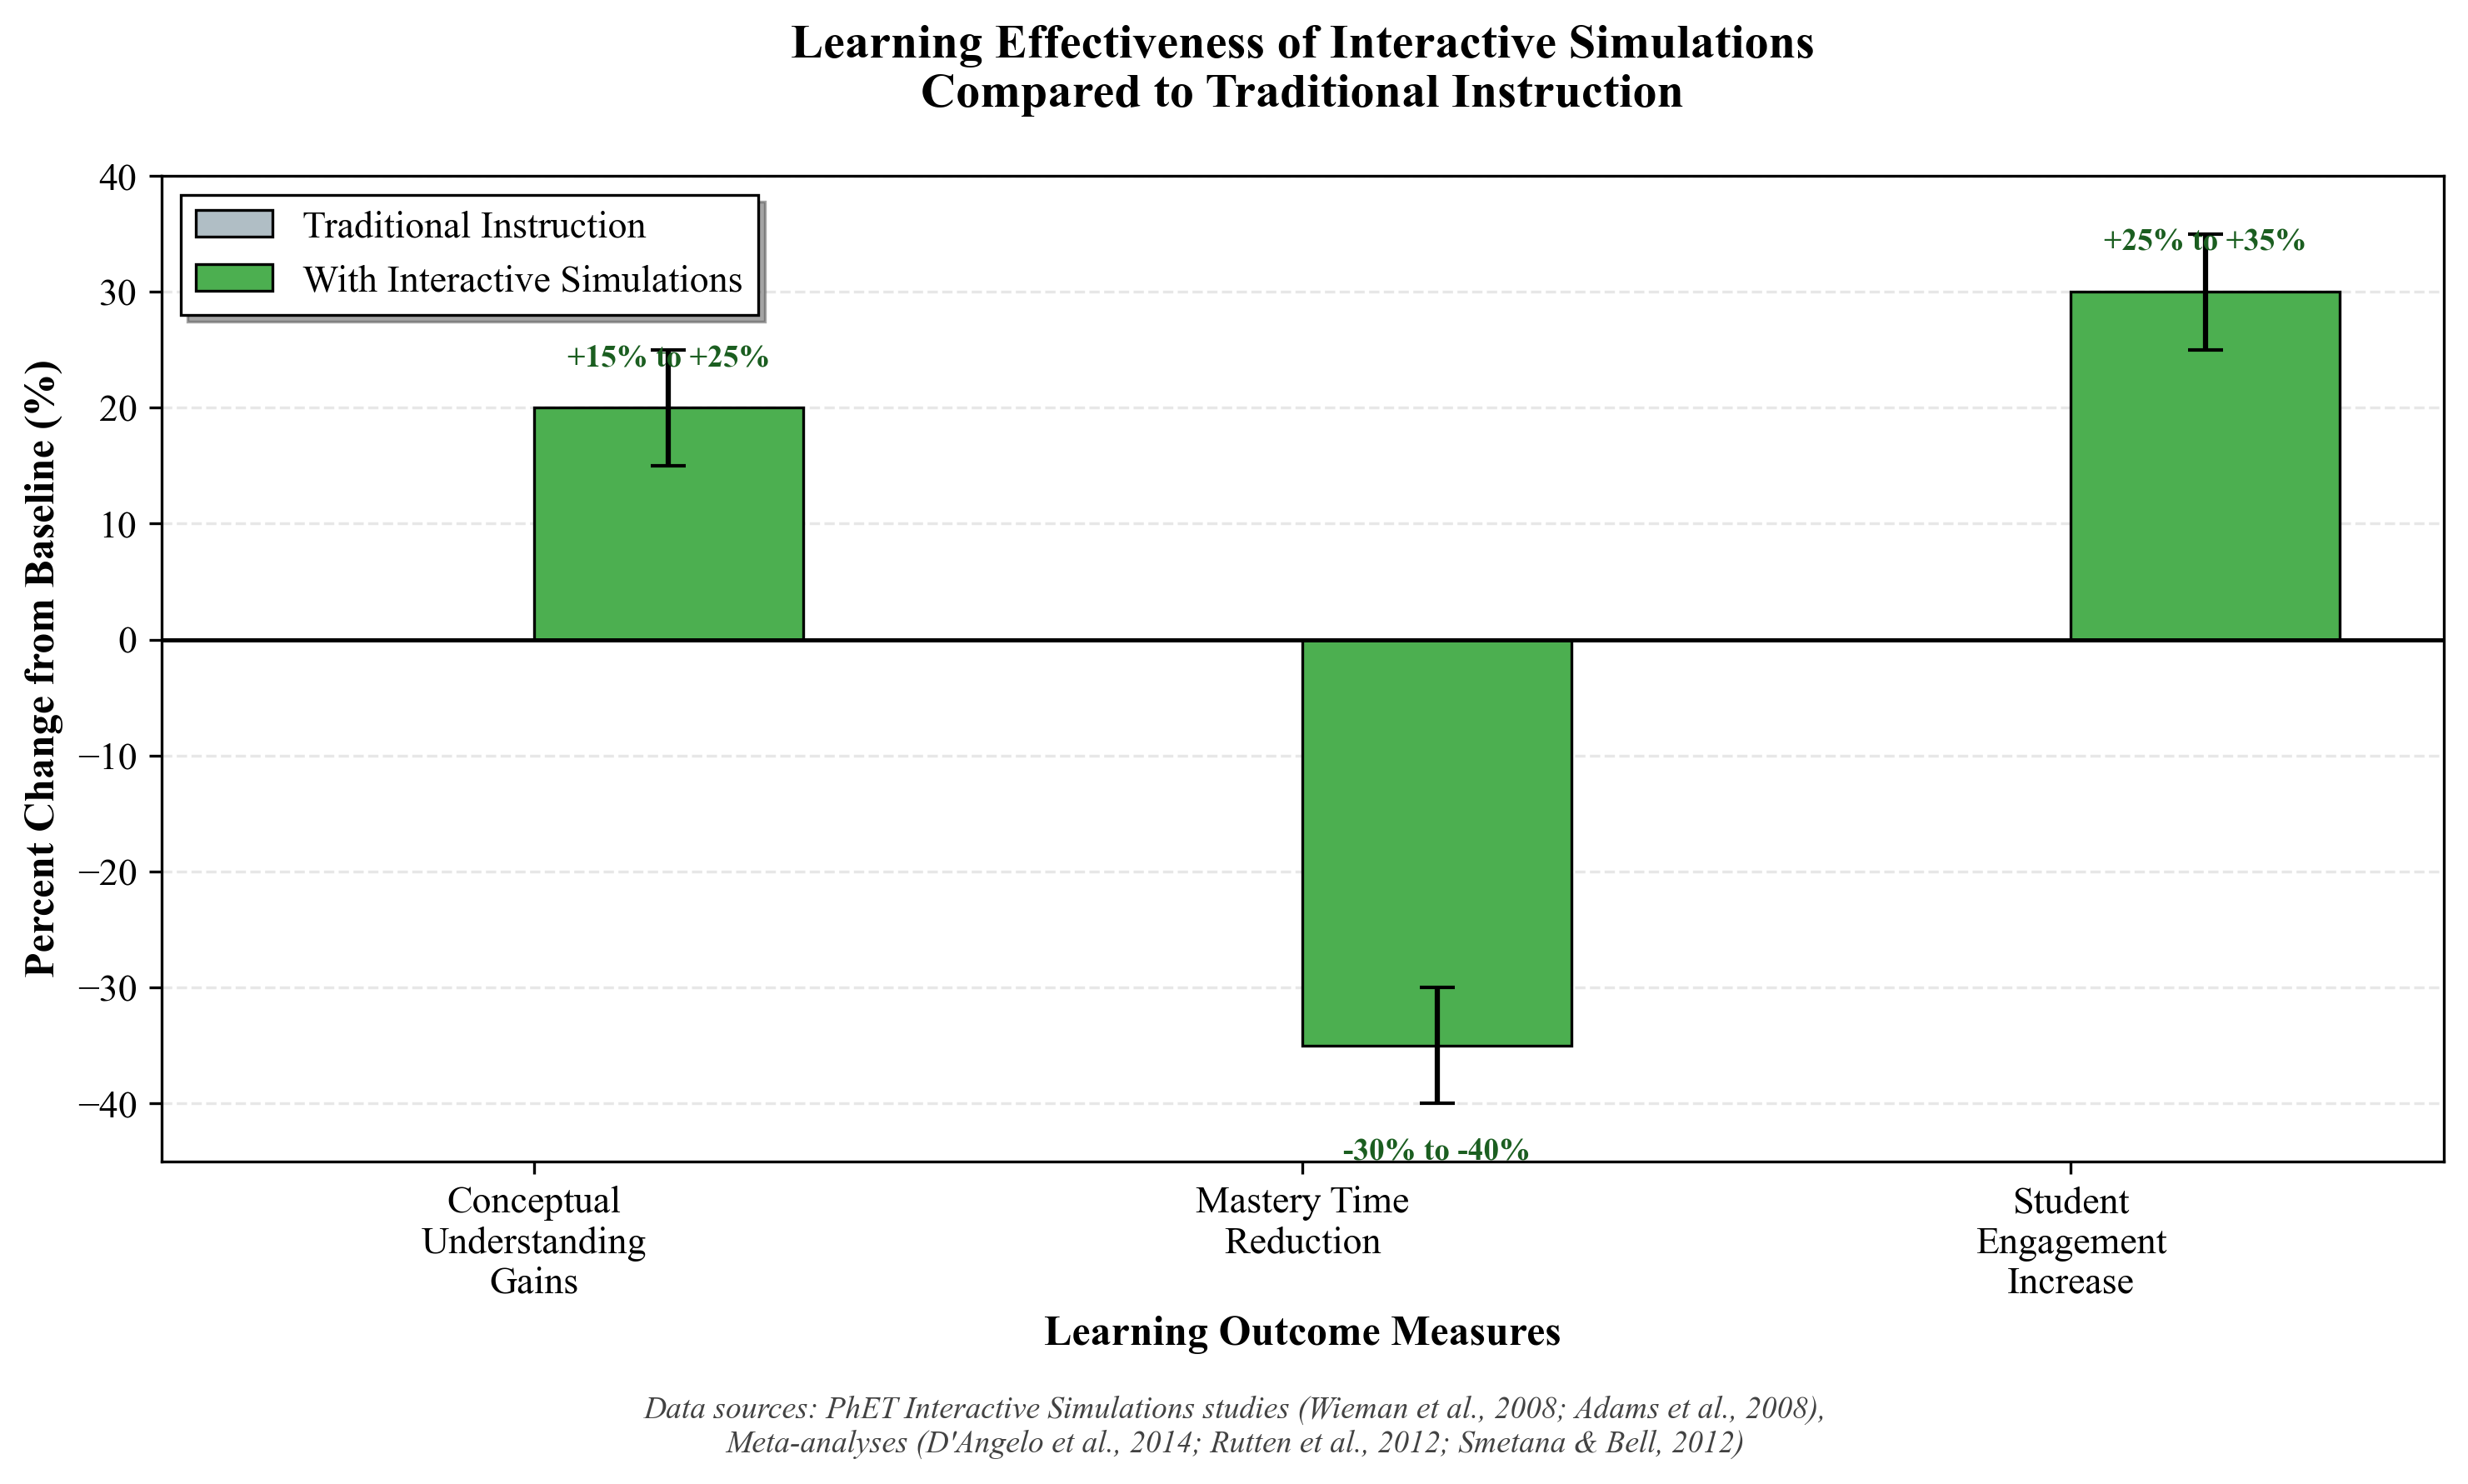
\includegraphics[width=0.95\textwidth]{figures/effectiveness-chart.png}
\caption{Learning effectiveness of interactive simulations compared to traditional instruction across three key outcome measures. Data represent meta-analysis findings from multiple studies including PhET Interactive Simulations research and systematic reviews across STEM disciplines. Error bars indicate reported ranges of improvement. Sources: Wieman et al. (2008), Adams et al. (2008), D'Angelo et al. (2014), Rutten et al. (2012), Smetana \& Bell (2012).}
\label{fig:effectiveness}
\end{figure}

These impressive gains, visualized in Figure~\ref{fig:effectiveness}, reflect simulations' ability to make abstract concepts tangible and provide immediate, interactive feedback that supports active learning. By allowing learners to \textit{visualize invisible processes} such as magnetic fields, molecular motions, or electric currents, simulations bridge the gap between theoretical knowledge and real-world phenomena \cite{phet2023}.

\subsection{PhET Interactive Simulations: Evidence at Scale}

The PhET Interactive Simulations project at the University of Colorado Boulder provides the most comprehensive evidence for simulation effectiveness at scale. With over 45 million simulation runs annually across 175 countries, PhET represents one of the largest deployments of educational simulations worldwide \cite{phet2023}. This massive usage scale, combined with extensive research validation, demonstrates both the practical feasibility and educational effectiveness of well-designed interactive simulations.

Studies of PhET simulations have demonstrated significant learning gains across diverse populations and educational contexts \cite{adams2008study, finkelstein2005phet, perkins2006phet}. In controlled experiments comparing simulation-based instruction to traditional approaches, students using PhET simulations consistently achieved higher scores on conceptual assessments and demonstrated superior long-term retention.

\textbf{Controlled Experimental Evidence}: In a particularly compelling controlled study, high school physics students were randomly assigned to learn circuit concepts using either PhET Circuit Construction Kit simulations or physical circuit equipment (wires, bulbs, resistors). Despite equivalent instructional time and support, students using the simulation significantly outperformed their peers who used physical equipment on subsequent conceptual exam questions. Most remarkably, six weeks after the initial instruction, the simulation group demonstrated substantially better knowledge retention, suggesting that the interactive visual feedback provided by the simulation created more durable mental models \cite{finkelstein2005phet}.

\textbf{Transfer to Physical Skills}: Perhaps most surprising, when both groups were eventually asked to construct physical circuits with real equipment, students initially trained on simulations performed the task faster and with greater confidence than those who had originally used physical apparatus. This finding challenges the common assumption that virtual experiences cannot adequately prepare students for hands-on tasks, instead suggesting that well-designed simulations can provide superior conceptual foundations that transfer effectively to practical applications \cite{finkelstein2005phet}.

\textbf{Classroom Implementation Patterns}: Survey research with hundreds of PhET-using educators reveals that teachers employ simulations flexibly across diverse pedagogical contexts: demonstrations during lectures, guided inquiry laboratory activities, homework assignments, and remediation for struggling students. The primary goals educators report for using simulations include developing conceptual understanding, promoting scientific inquiry skills, and addressing known misconceptions \cite{phet2023}.

\subsection{How Students Interact with MicroSims}

Understanding how students actually engage with interactive simulations illuminates why these tools prove effective and what design principles support productive learning interactions. Research based on classroom observations, student interviews, and interaction logging provides detailed insights into the phenomenology of simulation-based learning.

\subsubsection{Guided Exploration and Playful Experimentation}

Students typically interact with effective simulations through a combination of guided exploration and playful experimentation. Well-designed simulations employ \textit{intuitive interfaces} with minimal text requirements, familiar object representations, and direct manipulation controls that enable learners of various ages to begin exploring immediately. PhET simulations exemplify this design philosophy by using everyday objects such as light bulbs, beakers, and bicycles as interface icons, helping students connect scientific concepts to prior knowledge and lived experience \cite{phet2023}.

As students manipulate simulation parameters through sliders, buttons, and direct object manipulation, the simulation provides instant animated feedback that makes cause-and-effect relationships immediately visible. This interactivity invites learners to pose "What if..." questions and observe consequences in real time, fostering hypothesis generation and empirical testing behaviors characteristic of scientific thinking.

Classroom observations reveal a distinctive interaction pattern: students often engage in initial playful exploration, manipulating controls with apparent randomness, then gradually focus attention on underlying scientific principles as they notice systematic patterns and regularities. This progression from play to focused inquiry appears to be pedagogically productive, as the initial exploratory phase builds familiarity with the simulation interface and generates questions that motivate subsequent systematic investigation \cite{phet2023}.

\subsubsection{The Critical Role of Scaffolding}

The level of instructional guidance accompanying simulations significantly influences the depth and quality of student engagement. Research comparing different activity structures reveals that both extremes---highly prescriptive step-by-step procedures and completely unguided free exploration---produce suboptimal learning outcomes \cite{phet2023}.

Overly structured activities that specify every action and observation lead to shallow, procedure-following behavior where students complete tasks without developing genuine conceptual understanding. Students in such contexts often focus on obtaining the "correct answer" rather than exploring the underlying phenomena or constructing their own understanding.

Conversely, completely unguided exploration can leave students overwhelmed by the simulation's possibility space, uncertain what aspects merit attention, and unable to connect their observations to relevant scientific principles. Without some strategic direction, many students may never discover the simulation's most pedagogically significant features or recognize the conceptual importance of particular phenomena.

The optimal approach identified by research provides \textit{minimal but strategic scaffolding}: a few well-designed open-ended questions or challenges that guide students toward investigating key features without dictating specific procedures. Such "gentle guidance" prompts might ask students to "find three ways to make the bulb brighter" or "predict what will happen when you double the voltage, then test your prediction" \cite{phet2023}.

This balanced scaffolding approach encourages self-directed inquiry where students form predictions, design tests, observe outcomes, and refine their understanding through iterative cycles. Students engaging in this guided-but-not-prescribed exploration demonstrate deeper conceptual reasoning than peers experiencing either overly structured or completely unstructured activities \cite{phet2023}.

\subsubsection{Collaborative Learning and Peer Discussion}

Classroom implementations frequently position simulations as collaborative activities where students work in pairs or small groups. This social configuration promotes productive peer discussion as students debate predictions, explain observations to one another, and collectively make sense of simulation behaviors. The collaborative context transforms individual cognitive engagement into social knowledge construction, with students challenging each other's misconceptions and collectively building more sophisticated understanding.

The simulations' visual, dynamic nature provides a shared referent for group discussion---students can point to specific elements on screen, propose interpretations of what they observe, and negotiate meaning through dialogue anchored in their common perceptual experience. This shared visual reference appears to scaffold productive scientific argumentation even among younger learners who might struggle with purely verbal scientific discourse.

\subsubsection{Safe Experimentation and Risk-Taking}

A consistently reported benefit of simulation-based learning is that virtual environments eliminate risks associated with physical experimentation. Students demonstrate greater willingness to try unconventional approaches, test extreme parameter values, and recover from "failures" when working with simulations compared to physical equipment \cite{phet2023}.

One revealing study contrasted students' affective responses when using circuit simulations versus real circuit equipment. Students working with physical apparatus expressed nervousness about breaking expensive equipment or injuring themselves, leading to cautious, conservative exploration strategies. In contrast, students using the Circuit Construction Kit simulation "explored and investigated without needing much assistance," trying diverse configurations and learning through trial and error without anxiety about consequences \cite{finkelstein2005phet}.

This psychological safety appears particularly valuable for students from groups traditionally underrepresented in STEM fields, who may experience heightened anxiety about appearing incompetent or damaging equipment. By removing performance pressure and material consequences, simulations can provide more equitable access to exploratory learning experiences.

\subsection{Effectiveness Across Grade Levels}

One of the most significant advantages of well-designed interactive simulations is their pedagogical effectiveness across diverse educational levels, from upper elementary school through higher education. This adaptability enables the same fundamental design principles to support age-appropriate learning across a remarkably wide developmental span.

\subsubsection{Elementary Education (Grades 3-5)}

Research demonstrates that even young learners aged 10-12 can benefit substantially from appropriately designed simulations. In one longitudinal study, fifth and sixth grade students used an ecosystem simulation over multiple class sessions and demonstrated "considerable improvements" in systems thinking skills, including understanding of ecological processes and interactions \cite{eric2009}. This evidence challenges assumptions that complex system modeling exceeds young learners' capacities, suggesting instead that well-designed simulations can scaffold sophisticated thinking even in elementary contexts.

Effective simulations for this age group employ simpler interfaces, more scaffolding guidance, and contexts tied to students' everyday experiences. Visual design typically employs cartoon-style graphics and anthropomorphized representations that appeal to younger learners while maintaining scientific accuracy. The content focus remains on foundational concepts presented through familiar scenarios---for example, exploring food webs through animals students recognize, or investigating basic physics through playground equipment simulations.

Despite the relative scarcity of research on elementary-level simulation use, existing evidence suggests substantial potential impact. As one systematic review noted, this scarcity represents a significant gap and opportunity: developing more MicroSims targeting K-5 curriculum standards could yield considerable benefits, particularly for schools lacking hands-on science resources \cite{mdpi2024}.

\subsubsection{Middle School (Grades 6-8)}

Middle school students, with their developing capacity for abstract reasoning, readily engage with simulations addressing introductory physics, earth science, pre-algebra, and life science topics. This developmental stage represents an optimal window for simulation-based instruction, as students can handle moderately complex interfaces while still benefiting from visual, interactive representations of abstract concepts.

Research at this level demonstrates simulations' effectiveness for addressing common misconceptions that emerge as students begin formal study of scientific phenomena. For example, simulations addressing force and motion help students overcome prevalent Aristotelian misconceptions about objects in motion, while chemistry simulations addressing particulate models of matter challenge students' intuitive but incorrect ideas about dissolving and chemical reactions.

\subsubsection{High School (Grades 9-12)}

At the high school level, simulations become integral components of rigorous STEM courses. Physics, chemistry, and biology courses routinely employ simulations both as alternatives to physical laboratory experiments and as unique learning tools that enable investigations impossible with physical equipment. Survey research reveals that high school and college instructors often use identical PhET simulations but adapt the surrounding activities and expectations to match student developmental levels \cite{phet2023}.

High school simulations can incorporate quantitative analysis, complex parameter spaces, and open-ended investigation designs that challenge advanced students while remaining accessible through intuitive visual interfaces. Students at this level increasingly use simulations for homework and independent study, indicating that well-designed tools can support self-directed learning outside formal classroom contexts.

\subsubsection{Higher Education}

At the college and university level, simulations support sophisticated conceptual understanding in introductory courses while also serving specialized functions in advanced coursework. In large-enrollment introductory courses, simulations provide active learning experiences that would be logistically impossible with physical equipment given typical class sizes and resource constraints.

For more advanced courses, simulations enable exploration of phenomena that would require specialized, expensive equipment (such as quantum mechanical systems or high-energy particle interactions) or dangerous procedures (such as chemical reactions involving hazardous materials). Graduate-level simulations may incorporate research-grade models and extensive parameter customization, blurring the boundary between educational tools and research instruments.

\textbf{Summary Across Levels}: While specific implementations vary by educational level, several core benefits remain consistent across all age groups: simulations make learning interactive and visual, provide immediate feedback, enable safe experimentation, and transform abstract concepts into manipulable experiences. The primary differences involve interface complexity, conceptual sophistication, and the degree of instructional scaffolding provided. This developmental continuity suggests that establishing simulation literacy early---through elementary and middle school experiences---prepares students to leverage increasingly sophisticated simulation-based learning as they advance through their education.

\subsection{Common Characteristics of Effective MicroSims}

Research on simulation effectiveness identifies several key design characteristics that consistently correlate with improved learning outcomes. These characteristics should inform development of new educational simulations and provide evaluation criteria for assessing existing resources.

\textbf{Intuitive, Student-Friendly Interfaces}: Effective simulations employ clean visual designs, minimal text requirements, and familiar metaphors that enable students to begin productive exploration without extensive instruction. Controls utilize standard interaction paradigms (dragging, sliding, clicking) and respond instantly, creating smooth dialogues between student actions and simulation feedback \cite{phet2023}. Intuitive design minimizes extraneous cognitive load, allowing learners to focus mental resources on scientific content rather than interface navigation.

\textbf{Familiar Contexts and Analogies}: The most pedagogically effective simulations depict scenarios or objects that students recognize from everyday experience: bicycles, balloons, magnets, kitchen utensils. This contextualization in familiar situations helps students activate relevant prior knowledge and form connections between scientific principles and lived experience \cite{phet2023}. Analogies embedded within simulations---such as modeling electric current flow using water flow---further aid conceptual understanding by connecting unfamiliar scientific phenomena to more intuitive physical systems.

\textbf{Making the Invisible Visible}: Perhaps the most distinctive pedagogical affordance of interactive simulations is their capacity to visualize normally invisible processes. Effective simulations render visible the phenomena students must understand but cannot directly observe: electrons moving through circuits, molecules colliding during chemical reactions, magnetic fields extending through space, quantum wave functions evolving over time \cite{phet2023, finkelstein2005phet}.

Many high-quality simulations provide multiple linked representations---for example, showing both a macroscopic view of a chemical reaction and a molecular-level animation simultaneously, or coordinating a physical simulation with real-time graphical plots of relevant variables. These coordinated representations help students construct connections between different levels of analysis and develop more integrated understanding \cite{phet2023}.

\textbf{Interactive and Responsive Feedback}: High-quality simulations provide immediate, dynamic responses to every student action. When learners adjust a slider, add an object, or change a parameter value, the simulation responds instantly with animated changes, updated graphs, and modified outcomes. This immediacy reinforces cause-and-effect relationships and supports learning through exploration and experimentation \cite{phet2023}.

Effective simulations also incorporate productive constraints---boundaries on possible actions that focus attention on scientifically relevant phenomena without overtly prescribing student behavior. For example, a circuit simulation might physically prevent impossible connections while allowing all valid circuit configurations, subtly guiding students toward productive exploration without explicitly instructing them what to try.

\textbf{Appropriate Challenge and Scaffolding}: The most effective simulations achieve a careful balance between ease of use and intellectual challenge. They often include implicit puzzles or goal-oriented tasks---such as achieving a stable orbit in a gravity simulation or lighting a bulb with limited circuit components---that spark curiosity and motivate exploration \cite{phet2023}.

Simultaneously, simulations must remain accessible through intuitive controls and clear visual feedback that prevent frustration. Many successful simulations accompany their open-ended design with optional hints, guiding questions, or progressive complexity levels that provide scaffolding for struggling students while remaining unobtrusive for those who prefer independent exploration.

\textbf{Research-Tested and Refined}: A distinguishing feature of the most effective educational simulations is that they undergo extensive iterative testing and refinement driven by education research. PhET simulations exemplify this approach, with each simulation progressing through multiple development cycles involving student interviews, classroom observations, and systematic assessment of learning outcomes \cite{phet2023}.

This research-based refinement process results in simulations that effectively target known misconceptions, provide intuitive interfaces that align with student thinking, and include design features specifically engineered to promote correct conceptual understanding. The documented effectiveness of research-tested simulations underscores the importance of evidence-based design processes rather than relying solely on designer intuition or general software engineering principles.

\subsection{High-Impact Application Categories}

Based on extensive research and documented effectiveness, several categories of interactive simulations emerge as particularly high-impact for STEM education. These domains represent areas where simulations provide unique pedagogical value and where continued development efforts promise substantial educational returns.

\subsubsection{Physics and Engineering}

Physics has proven extraordinarily fertile ground for educational simulations, given the field's abstract concepts and often-invisible forces. Simulations covering classical mechanics (motion, gravity, energy conservation), electromagnetism (circuits, fields, magnetism), waves (sound, light, interference), and modern physics (quantum phenomena, relativity) have demonstrated consistently strong impacts on student learning \cite{wieman2008phet, finkelstein2005phet}.

Physics simulations enable students to visualize forces and fields, manipulate time scales to slow motion or observe long-term system evolution, and experiment with parameter values impossible to achieve or isolate in physical laboratory settings. Circuit simulations, for example, allow students to observe charge flow directly and instantly reconfigure connections, leading to superior conceptual understanding compared to using physical wires and components \cite{finkelstein2005phet}.

Engineering-oriented simulations provide sandbox environments for design and experimentation, enabling students to construct bridges, design electrical systems, or optimize mechanical devices through iterative testing without material costs or safety concerns. These simulations develop both domain knowledge and design thinking skills essential for engineering practice.

Future development priorities in this category include simulations for advanced topics that are particularly difficult to demonstrate in traditional classrooms: magnetic field interactions, semiconductor physics, relativistic effects, and quantum mechanics visualizations. Such simulations could make typically abstract and mathematically intensive content more accessible and intuitive for broader student populations.

\subsubsection{Chemistry and Molecular Science}

Chemistry simulations possess unique power to transport students into the molecular realm, making visible the atomic and molecular processes underlying macroscopic chemical phenomena. High-impact examples address chemical bonding, reaction mechanisms, equilibria, gas laws, solutions and pH, and atomic structure \cite{phet2023}.

Effective chemistry simulations typically feature multiple coordinated representations: molecular animations showing individual particles alongside macroscopic views and graphical plots of concentration, energy, or other relevant variables. These linked representations help students construct connections between molecular behaviors and observable chemical properties---a notoriously difficult conceptual leap in chemistry education \cite{phet2023}.

Chemistry simulations also provide virtual laboratory environments for experiments that would be dangerous, expensive, or time-consuming with physical materials. Students can explore reaction kinetics by instantly adjusting temperature or try numerous reactant combinations without safety concerns or material costs. The ability to observe molecular collision dynamics and reaction mechanisms provides insights impossible to achieve through physical laboratory work.

Research indicates that molecular-level simulations effectively address common misconceptions about dissolving, phase changes, and chemical reactions while improving overall conceptual understanding in chemistry courses \cite{mdpi2024}. Developing additional simulations for under-represented topics such as organic reaction mechanisms, electrochemistry, and environmental chemistry processes could substantially enhance chemistry education accessibility and effectiveness.

\subsubsection{Biology and Life Sciences}

In biological sciences, simulations model processes occurring within organisms and ecosystems, often involving time scales and spatial scales difficult to observe directly. Cell and molecular biology simulations addressing gene expression, cellular respiration, and protein synthesis enable students to manipulate biological pathways and observe consequences, supporting understanding of complex biochemical sequences \cite{mdpi2024}.

Human anatomy and physiology simulations provide interactive models of body systems---circulatory, nervous, digestive---that are more ethical and often more informative than traditional dissection while remaining highly engaging for students. The ability to highlight specific components, show invisible processes like nerve signal transmission, and manipulate physiological parameters provides learning experiences impossible through physical specimens.

At larger scales, ecology and environmental science simulations model population dynamics, predator-prey relationships, disease transmission, and climate systems. These simulations allow students to experiment with ecological parameters and observe long-term consequences in accelerated time, promoting systems thinking by revealing how changes in one system component cascade through interconnected networks \cite{eric2009}.

One elementary-level study using an ecosystem simulation found substantial improvements in students' systems thinking skills, including understanding of processes, interactions, and ecological relationships. However, the study also identified persistent difficulties with feedback loops and cyclical causation, suggesting that further simulation design innovation is needed to effectively scaffold understanding of these complex system dynamics \cite{eric2009}.

Biology simulations prove particularly engaging because they connect to personally relevant topics---health, environment, organisms students encounter---and often incorporate game-like scenarios such as maintaining ecological balance or preventing disease outbreaks. Expanding simulation resources for genetics, evolution, microbiology, and complex ecosystem modeling represents a high-priority development area likely to yield significant educational impact.

\subsubsection{Mathematics and Computational Thinking}

Mathematics-focused simulations help students visualize abstract mathematical concepts by transforming them into interactive, manipulable objects. Examples span from elementary-level simulations exploring fractions through adjustable visual representations to advanced mathematics involving function transformations, multivariable calculus, and linear algebra.

Algebra and geometry simulations enable learners to manipulate equations or geometric objects and immediately observe resulting changes, reinforcing concepts such as slope, transformations, congruence, and similarity through dynamic visual feedback. Probability and statistics simulations allow students to conduct virtual experiments with thousands of trials in seconds, building intuition about randomness, sampling distributions, and statistical inference that would be impractical to develop through physical experiments.

While mathematics simulations have received less research attention than science simulations, platforms including PhET offer numerous mathematics-focused tools, and educator reports indicate positive impacts on engagement and conceptual understanding. Connecting mathematical concepts to visual, manipulable representations appears particularly beneficial for students who struggle with purely symbolic mathematical notation.

Computational thinking and computer science concepts can also be taught through carefully designed simulations: guiding virtual robots through mazes to teach programming logic, visualizing sorting algorithms, or manipulating data structures. As computational thinking becomes increasingly central to K-12 curricula, simulation-based approaches offer accessible entry points for students without prior programming experience.

Future development priorities include simulations for calculus concepts (such as interactive integral visualization accumulating area), linear algebra (visualizing vector spaces and matrix transformations), and applied mathematics contexts (financial modeling, engineering applications) that demonstrate real-world relevance while building mathematical understanding.

\subsubsection{Complex Systems and Systems Thinking}

This cross-disciplinary category addresses one of education's most significant challenges: developing students' capacity to understand complex, dynamic systems with multiple interconnected components. Systems thinking simulations model phenomena characterized by feedback loops, time delays, emergent behaviors, and non-obvious cause-effect relationships \cite{eric2009}.

Examples include environmental systems (climate models, water resource management), socio-economic systems (urban development, economic models), and integrated science issues (energy grids combining physics, economics, and environmental factors). Such simulations allow students to manipulate system components and observe cascading effects, teaching them to think in terms of stocks, flows, delays, and feedback loops rather than simple linear causation.

Research with ecosystem simulations for middle school students demonstrated improvements in understanding system structures and component interactions, but also revealed persistent difficulties with feedback loops and cyclical causation \cite{eric2009}. These findings suggest both the promise and challenge of systems thinking education: simulations can effectively scaffold certain aspects of systems thinking, but current designs may require enhancement to adequately address the most conceptually difficult elements of complex systems.

High-impact systems simulations effectively visualize flows of conserved quantities (energy, matter, money, population) and accumulate changes over time through graphical displays. They encourage what-if analysis, positioning students as decision-makers exploring policy consequences: "What happens if we increase recycling rates by 50\%? What if we introduce a new predator species?"

Causal loop diagrams, stock-and-flow models, and system dynamics simulations help students recognize circular causation, time delays, and system equilibria---essential concepts for understanding global challenges involving climate, resources, public health, and social systems. Given the importance of systems thinking for addressing complex real-world problems, continued development of accessible, pedagogically effective simulations in this category represents a high-priority investment likely to yield substantial educational and societal returns.

\subsection{Subject Areas Requiring Specialized Supporting Libraries}

While p5.js provides an excellent foundation for many educational simulations, certain subject areas require specialized visualization or interaction libraries to achieve maximal pedagogical effectiveness. Identifying these areas and developing appropriate supporting libraries represents an important priority for expanding MicroSim capabilities across the full curriculum.

\subsubsection{History and Geography}

Historical and geographical education benefit tremendously from timeline and mapping visualizations that contextualize events spatially and temporally. However, creating effective interactive timelines and geographic visualizations requires specialized libraries beyond p5.js core capabilities.

\textbf{Timeline Visualizations}: Libraries such as vis-timeline.js enable creation of interactive historical timelines where students can explore event sequences, understand historical periods, and recognize concurrent developments across different regions or domains. Educational applications include comparing technological developments across civilizations, understanding cause-and-effect sequences in historical events, and recognizing patterns in historical change. High-quality timeline templates incorporating pedagogical best practices would significantly lower barriers to creating history-focused MicroSims.

\textbf{Geographic Mapping}: Libraries like Leaflet.js provide interactive mapping capabilities essential for geography, environmental science, and social studies education. Geographic simulations could enable students to explore resource distribution, understand migration patterns, investigate environmental changes, or analyze geopolitical relationships. Integrating mapping libraries with MicroSim design patterns while maintaining the framework's simplicity and generative AI compatibility represents an important technical challenge with substantial educational payoff.

\subsubsection{Electrical Circuits and Signal Processing}

Circuit education presents unique challenges requiring specialized component libraries for drawing schematic diagrams, simulating circuit behavior, and animating current flow. While PhET's Circuit Construction Kit demonstrates the pedagogical value of interactive circuit simulations, creating new circuit simulations currently requires substantial specialized programming.

\textbf{Circuit Schematic Components}: A comprehensive p5.js circuit drawing library providing standard electrical components (resistors, capacitors, batteries, switches, transistors) with appropriate connection logic would enable rapid development of circuit-focused MicroSims. Such a library should handle component placement, connection validation, and visual rendering while exposing circuit state for educational visualization.

\textbf{Current Animation}: Animating electron flow or current direction provides crucial visual feedback for understanding circuit behavior. A supporting library providing current animation capabilities---showing moving charges, indicating direction, and responding to circuit modifications---would substantially enhance circuit simulation pedagogical effectiveness.

\textbf{Signal Processing}: Related applications in signal processing, communications, and electrical engineering would benefit from libraries supporting waveform visualization, frequency analysis, and filter design. Enabling students to interactively explore Fourier analysis, modulation schemes, or digital signal processing through well-designed simulations could significantly improve accessibility of these mathematically intensive topics.

\subsubsection{Systems Dynamics and Causal Loop Diagrams}

Teaching systems thinking benefits from specialized visualization tools for stock-and-flow diagrams and causal loop diagrams. These representations help students understand accumulation, feedback loops, and circular causation in complex systems \cite{eric2009}.

A library supporting creation and interactive manipulation of causal loop diagrams would enable students to construct, test, and refine their own system models, promoting deeper engagement with systems thinking concepts. Such a library should support standard systems dynamics notation while remaining accessible for middle school through university students.

\subsection{Limitations and Challenges}

Despite their demonstrated effectiveness, educational simulations face several important limitations and challenges that must be acknowledged and addressed through ongoing research and development.

\textbf{Scope Constraints}: The deliberately focused nature of MicroSims means individual simulations cannot address all learning objectives within a domain. Complex, multi-faceted concepts may require sequences of simulations or complementary instructional approaches. Educators must thoughtfully integrate simulations within broader curriculum frameworks rather than viewing them as comprehensive, standalone educational solutions.

\textbf{Abstraction and Simplification}: By necessity, simulations simplify reality to make phenomena comprehensible and computable. While these simplifications often serve legitimate pedagogical purposes, they risk creating misconceptions if students do not understand model limitations. Simulations should explicitly document their assumptions and help students recognize that models are useful approximations rather than complete representations of reality.

\textbf{Technology Access and Digital Divide}: While browser-based simulations reduce technology barriers compared to specialized software, they still require reliable internet access and functional computing devices. Socioeconomic disparities in technology access risk making simulation-based learning another dimension of educational inequality unless intentionally addressed through school technology provisioning and alternative access strategies.

\textbf{Quality Variability}: Not all simulations prove equally effective. Poorly designed simulations can confuse rather than clarify, promote misconceptions, or simply fail to engage students productively. The demonstrated success of research-tested simulations like PhET underscores the importance of evidence-based design and iterative refinement. However, the MicroSims framework's goal of enabling rapid AI-assisted generation introduces quality assurance challenges requiring systematic approaches to validation and improvement.

\textbf{Teacher Preparation and Support}: Effective simulation use requires thoughtful pedagogical integration. Teachers need support in selecting appropriate simulations, designing accompanying activities with optimal scaffolding levels, and facilitating productive classroom discussions around simulation experiences. Professional development and high-quality instructional materials represent essential infrastructure for realizing simulations' educational potential.

\textbf{Assessment Integration}: Evaluating learning from simulation experiences presents ongoing challenges. While simulations generate rich interaction data potentially valuable for formative assessment, translating simulation performance into meaningful learning evaluation remains underdeveloped. Embedding meaningful assessment within simulations while maintaining their lightweight character requires continued innovation.

\subsection{Intelligent Textbook Integration Example}

The MicroSims framework envisions simulations not as isolated educational resources but as integrated components of intelligent, adaptive learning systems. An intelligent textbook system demonstrates how simulations can function within broader educational ecosystems to provide personalized, data-driven learning experiences.

\textbf{Adaptive Content Sequencing}: An intelligent textbook incorporating MicroSims continuously assesses student understanding through interaction patterns, simulation performance, and embedded assessment items. Based on this ongoing evaluation, the system adaptively sequences content---determining when students have sufficiently mastered prerequisites to advance, when additional practice through simulation exploration would benefit learning, or when remediation through alternative representations might address persistent misconceptions.

\textbf{Personalized Simulation Selection}: Rather than presenting identical content to all students, an intelligent textbook can select from libraries of related simulations targeting the same concepts at different complexity levels or through different contextual framings. A student struggling with abstract mathematical representations might receive a simulation emphasizing concrete, everyday contexts, while an advanced student might encounter more sophisticated parameter spaces and quantitative analysis tasks.

\textbf{Learning Analytics and Feedback Loops}: Comprehensive logging of student interactions with embedded simulations---including time spent, parameters explored, challenges attempted, and errors made---provides rich data for learning analytics. Intelligent systems analyze these data streams to identify struggling students requiring intervention, recognize common misconceptions requiring instructional attention, and refine content recommendations based on observed effectiveness patterns.

\textbf{Integration with Reinforcement Learning}: Advanced implementations might employ reinforcement learning algorithms that treat simulation selection and sequencing as optimization problems: the system learns through trial and error which combinations of simulations, scaffolding levels, and timing produce optimal learning outcomes for different student profiles. Over time, such systems become increasingly effective at personalizing educational experiences as they accumulate data about what works for whom under what circumstances.

This vision of intelligent textbook integration positions MicroSims as essential building blocks for next-generation adaptive learning systems---systems that combine the engagement and interactivity of simulations with the personalization and continuous improvement capabilities of AI-driven education technology.

\section{Discussion}
\label{sec:discussion}

% TODO: Synthesize insights from:
% - docs/why/uniqueness.md (implications for educational equity)
% - docs/why/motivation.md (future directions)
% - docs/chapters/advanced-topics.md (future work)
% Key topics to address:
% - Implications for educational equity
% - Network effects of standardization
% - Limitations and challenges
% - Broader impact on educational technology
% - Scalability considerations
% - Quality control in AI-generated content
% - Integration with adaptive learning systems

\subsection{Implications for Educational Equity}

The unique characteristics of MicroSims have significant implications for educational equity:

\textbf{Reduced Cost Barriers}: Traditional educational software often requires expensive licenses, powerful hardware, or high-bandwidth internet connections. MicroSims, being lightweight and self-contained, can run on basic devices with minimal connectivity, making quality interactive content accessible to under-resourced schools and students.

\textbf{Language and Cultural Adaptation}: AI systems can generate MicroSims in different languages or adapt them for different cultural contexts on demand, without requiring separate development efforts for each market.

\textbf{Accessibility by Design}: Standardized patterns include accessibility features, ensuring that generated MicroSims support screen readers, keyboard navigation, and other assistive technologies.

\subsection{Network Effects and Standardization}

The standardized architecture of MicroSims creates powerful network effects as adoption increases. Each new MicroSim created following the framework patterns contributes to a growing ecosystem that benefits all users.

\subsection{Limitations and Challenges}

Despite their advantages, MicroSims face several limitations that warrant discussion:

\textbf{Scope Constraints}: The deliberately focused nature of MicroSims means they cannot address all learning objectives. Complex, multi-faceted concepts may require sequences of MicroSims or complementary instructional approaches.

\textbf{AI Generation Quality}: While generative AI has made remarkable progress, the quality of AI-generated MicroSims still requires human review and refinement to ensure pedagogical soundness and functional correctness.

\textbf{Assessment Integration}: Embedding meaningful assessment within MicroSims while maintaining their lightweight character presents ongoing challenges.

\subsection{Broader Impact}

The MicroSim framework has implications beyond individual simulation creation, potentially influencing how educational technology is conceptualized, developed, and deployed more broadly.

% Additional content to be extracted from source files

\section{Conclusion}
\label{sec:conclusion}

% TODO: Synthesize conclusions from all chapters
% Key points to address:
% - Summary of contributions
% - Unique value proposition (simplicity + accessibility + AI generation)
% - Impact on educational content creation
% - Addressing adoption barriers
% - Future research directions:
%   * Enhanced AI generation capabilities
%   * Adaptive difficulty adjustment
%   * Learning analytics integration
%   * Multi-user collaborative simulations
%   * Integration with VR/AR platforms
% - Call to action for educational technology community

This paper has introduced MicroSims, a comprehensive framework for creating lightweight, interactive educational simulations that address persistent barriers to widespread adoption of simulation-based learning. By occupying the unique intersection of simplicity, accessibility, and AI-generation capability, MicroSims enable educators worldwide to create custom, curriculum-aligned simulations on demand.

\subsection{Summary of Contributions}

We have presented:
\begin{enumerate}
\item A comprehensive design framework encompassing technical architecture, pedagogical principles, and user experience guidelines
\item Evidence that standardized patterns enable reliable AI-assisted generation
\item An iframe-based distribution model providing universal embedding across learning platforms
\item A metadata framework supporting discovery, personalization, and learning analytics
\item Empirical evidence from educational research demonstrating simulation effectiveness
\end{enumerate}

\subsection{Future Directions}

Several promising research directions emerge from this work:

\textbf{Enhanced AI Capabilities}: As language models continue to improve, future work should explore more sophisticated simulation generation, including adaptive difficulty adjustment and personalized content creation based on individual student performance data.

\textbf{Learning Analytics Integration}: Deeper integration with learning analytics systems could enable real-time adaptation of simulation parameters based on aggregate student interaction patterns.

\textbf{Collaborative Simulations}: Extending the framework to support multi-user, collaborative simulation experiences while maintaining the lightweight architecture.

\textbf{Immersive Technologies}: Exploring integration with virtual and augmented reality platforms while preserving the core principles of simplicity and accessibility.

\subsection{Conclusion}

MicroSims represent a paradigm shift in educational content creation, transforming simulation development from a specialized, resource-intensive process to an accessible, AI-assisted workflow available to any educator. By removing traditional barriers of cost, technical complexity, and platform dependence, MicroSims democratize access to interactive educational experiences. As generative AI continues to advance, the MicroSim framework provides a foundation for the next generation of adaptive, personalized learning systems.

The ultimate goal remains unchanged: creating learning experiences that inspire curiosity, build understanding, and empower students to apply knowledge in meaningful ways. MicroSims represent one step toward realizing the vision of truly adaptive, universally accessible educational technology that serves all learners effectively.


% Acknowledgments (optional)
\section*{Acknowledgments}
The author would like to thank the open-source p5.js community, the educational technology research community, and the contributors to the PhET Interactive Simulations project whose research has informed this work.

% References
\bibliographystyle{ieeetr}
\bibliography{sections/references}

\end{document}
